\documentclass{article}
    \usepackage{url}
    \usepackage{cite}
    \usepackage{float}   
    \usepackage{xcolor}
    \usepackage{lscape}
    \usepackage{amssymb}
    \usepackage{titling}
    \usepackage{pdfpages}
    \usepackage{enumitem}
    \usepackage{graphicx}
    \usepackage{hyperref}
    \usepackage{fancybox}
    \usepackage{fancyvrb}
    \usepackage{enumerate}
    \usepackage{pdflscape}
    \usepackage{afterpage}
    \usepackage[normalem]{ulem}
    \usepackage{listings,lstautogobble}    
    \usepackage[margin=0.8in]{geometry}
    \usepackage[nottoc,notlot,notlof]{tocbibind}
    \renewcommand\maketitlehookd{\vfill\null}
    \renewcommand\maketitlehooka{\null\mbox{}\vfill}

    \newcommand\backgroundimage{
        \put(-5,0){
        \parbox[b][\paperheight]{\paperwidth}{
        \vfill
        \centering
        %
\includegraphics[height=\paperheight]{Images/background.jpg}
        \vfill
    }}}

    % Stole code from: https://tex.stackexchange.com/questions/83882/how-to-highlight-python-syntax-in-latex-listings-lstinputlistings-command

    % Default fixed font does not support bold face
    \DeclareFixedFont{\ttb}{T1}{txtt}{bx}{n}{12} % for bold
    \DeclareFixedFont{\ttm}{T1}{txtt}{m}{n}{12}  % for normal

    \definecolor{deepblue}{rgb}{0,0,0.5}
    \definecolor{deepred}{rgb}{0.6,0,0}
    \definecolor{deepgreen}{rgb}{0,0.5,0}

    % SQL style for highlighting
    \lstdefinestyle{sql}{
        language=SQL,
        basicstyle=\small,
        commentstyle=\color{gray},
        otherkeywords={self},
        keywordstyle=\ttb\color{deepblue},
        stringstyle=\color{deepgreen},
        numbers=left,
        numberstyle=\small,
        breaklines=true,
        frame=tblr,
        showstringspaces=false,
        autogobble=true,
        rulecolor=\color{black}
        }

    \lstdefinestyle{sharpc}{
        language=[Sharp]C,
        aboveskip=2mm,
        belowskip=2mm,
        columns=flexible,
        basicstyle=\small,
        commentstyle=\color{gray},
        otherkeywords={self},
        keywordstyle=\color{deepblue},
        stringstyle=\color{deepgreen},
        emphstyle=\color{deepred},
        numbers=left,
        numberstyle=\small,
        breaklines=true,
        breakatwhitespace=true,
        frame=tblr,
        showstringspaces=false,
        autogobble=true,
        rulecolor=\color{black},
        emph={
            Dictionary,
            DataRow,
            DataTable,
            Receipt,
            Staff,
            Customer,
            Items,
            Office,
            OfficeLocation
            },
        }

    \graphicspath{ {Images/} }

    \title{EBUS3030 Assignment 2}
    \author{
        Stavros Karmaniolos 
        \texttt{c3160280@uon.edu.au}\\
        Jay Rovacsek
        \texttt{c3146220@uon.edu.au}\\
        Jacob Litherland
        \texttt{c3263482@uon.edu.au}\\
        Edward Lonsdale
        \texttt{c3252144@uon.edu.au}
    }
    \date{\today}
    \hypersetup{
    colorlinks=true,
    linkcolor=black,
    filecolor=magenta,      
    urlcolor=blue,
    citecolor=red,
    linktoc=section,
    }
    \pagenumbering{arabic}

    \newlist{legal}{enumerate}{10}
    \setlist[legal]{label*=\arabic*.}

    \begin{document}
    \lstset{style=sql}
    \AddToShipoutPicture{\backgroundimage}

    \begin{titlingpage}
        \maketitle
    \end{titlingpage}

    \tableofcontents

%%%%%%%%%%%%%%%%%
\newpage
%%%%%%%%%%%%%%%%%
    
% ------------------------------------------------------------------------------------------------ %
% ASSIGNMENT OUTLINE
% ------------------------------------------------------------------------------------------------ %

    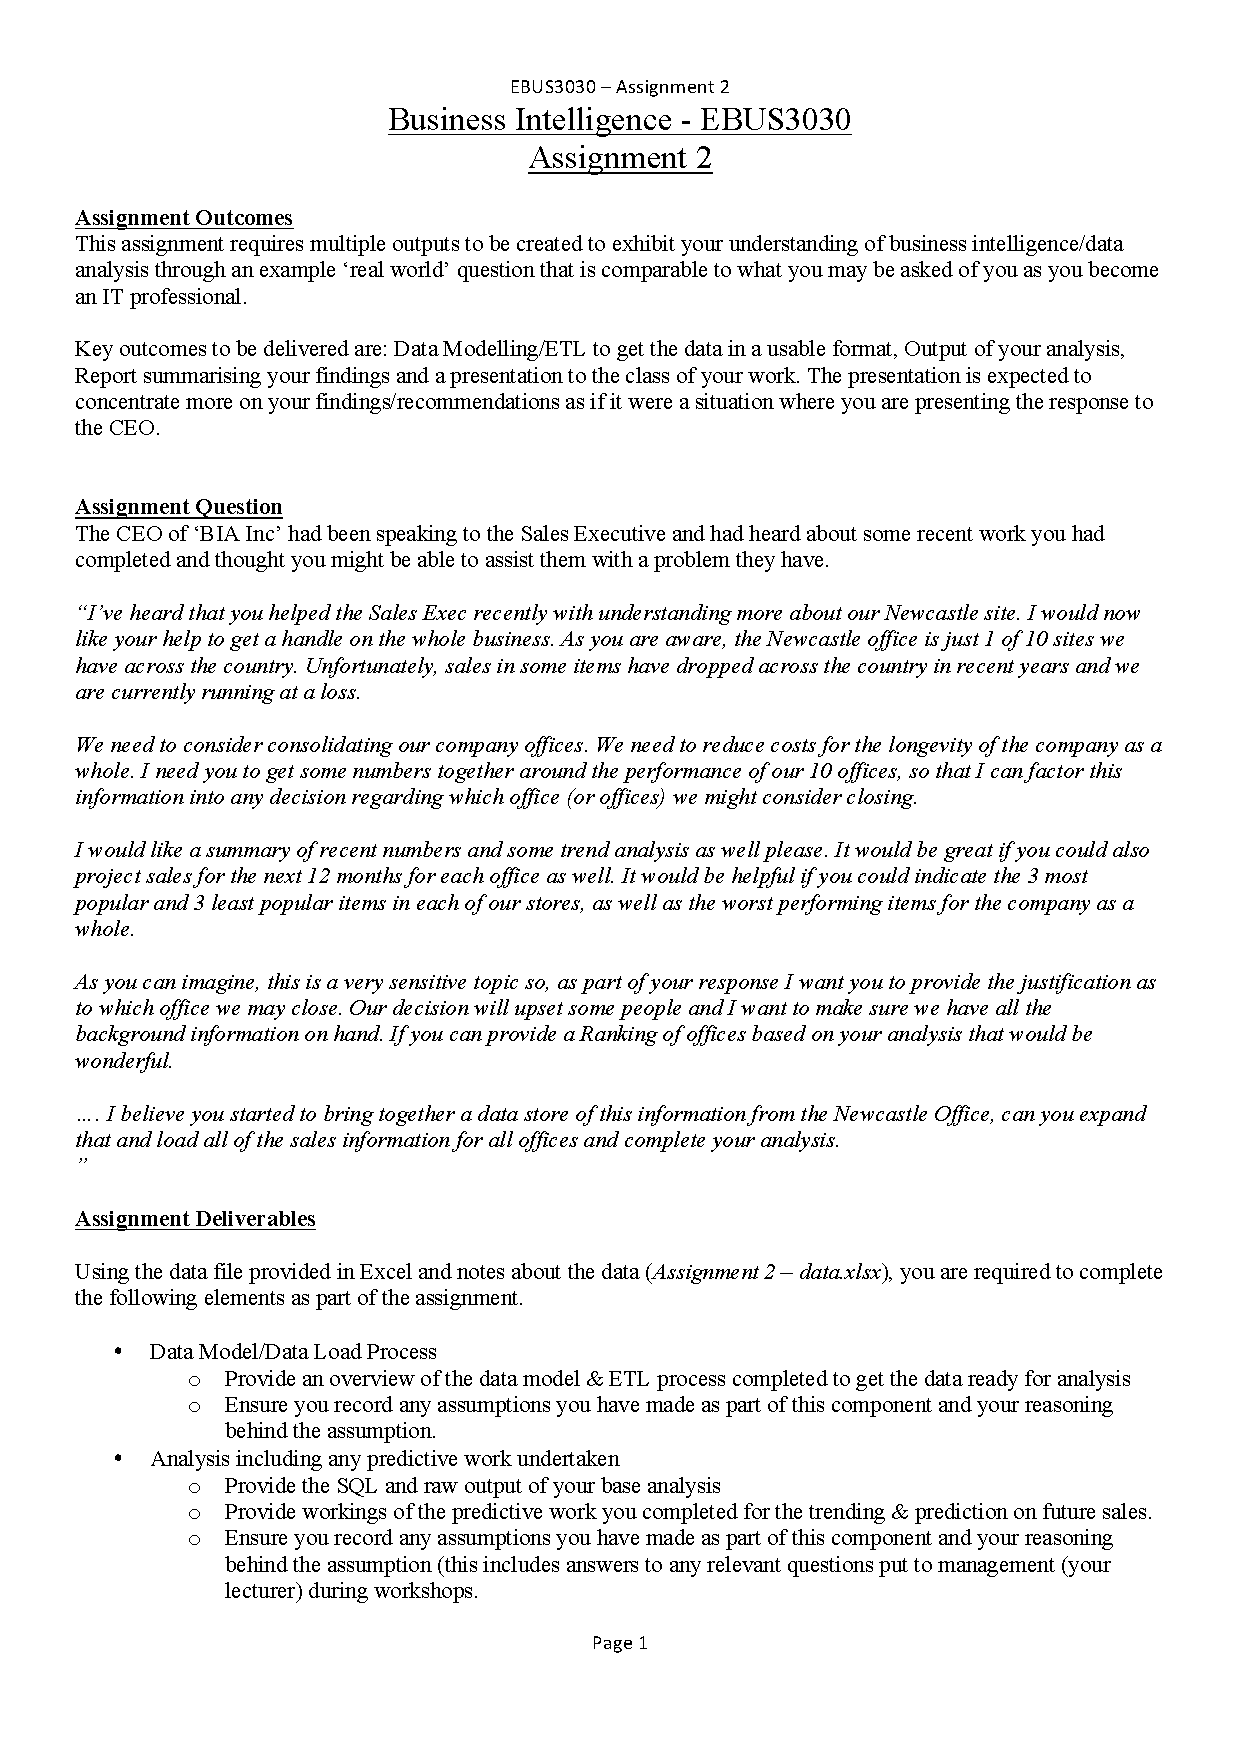
\includepdf[pagecommand=\section{Assignment Overview \& Requirements},width=\textwidth,keepaspectratio,pages={1}]{Resources/Assignment_2_Overview.pdf}
    \includepdf[width=\textwidth,keepaspectratio,pages={2}]{Resources/Assignment_2_Overview.pdf}

% ------------------------------------------------------------------------------------------------ %
% EXECUTIVE SUMMARY
% ------------------------------------------------------------------------------------------------ %

    \section{Executive Summary}
    \label{sec:Executive Summary}
	
%%%%%%%%%%%%%%%%%
\newpage
%%%%%%%%%%%%%%%%%


% ------------------------------------------------------------------------------------------------ %
% BUSINESS RULES
% ------------------------------------------------------------------------------------------------ %

    \subsection{Datamart Business Rules}
    The following business rules were provided to be used in the context of this assignment:
    \begin{itemize}
        \item At BIA all customers interacts are in an online environment.We only support electronic orders.
        \item Returning Customers can provide POI information via the web interface and look up their record 
        and that will flow with the sale
        \item The sales associate can complete the order form/sale for the client.
        \item Each sale will have a receipt number/id.
        \item A receipt can have many line items 
        \item Each line item can only be for a single item, but the customer can purchase multiples of the same item.
        \item After consultation with your team, we have made the following change to discount applied to sales: 
        Where a customer has multiple line items, any sale with 5 or more row items (containing at least 5 different items) 
        is provided a 5\% discount.
        \item The system automatically handles the total for the sale by looking up the item, then multiplying the costs 
        per item by number purchased, and then should store this final field total as a record in the system (but should
        also be able to see clearly sales that were provided a discount. 
        \item Store Item prices can change at any point, however the price the customer pays is the amount listed for the
        store item that is sold on the sale date. We need to keep a record of all store item prices historically so that 
        we can determine what the store item price was at any particular past date.
        \item Only one BIA sales assistant can be attributed to any receipt.
        \item Customers may visit multiple stores for purchases (ie they are not locked to a particular store). As a 
        result, all customer records are replicated across all stores, so they do not need to be re-recorded at a 
        store by store level.
    \end{itemize}
   
    With these considerations in mind, the following report was created to outline
    the discovery, creation and polish to satisfy the assignment requirements.

% ------------------------------------------------------------------------------------------------ %
% DATA MODEL
% ------------------------------------------------------------------------------------------------ %

%%%%%%%%%%%%%%%%%
\newpage
%%%%%%%%%%%%%%%%%

    \section{Data Model}
    
    	The following section outlines the models used in the design and creation of the database. It includes the EER Model with relations, attributes and relationships as well as the database schema from Microsoft SQL Server Management Studio.
    
        \subsection{Database Schema}
            The below data model is only a suggestion and is still subject to change into the future. A full create script can be found in the \hyperref[sec:Appendix]{\color{blue}appendix}
                \begin{center}
                    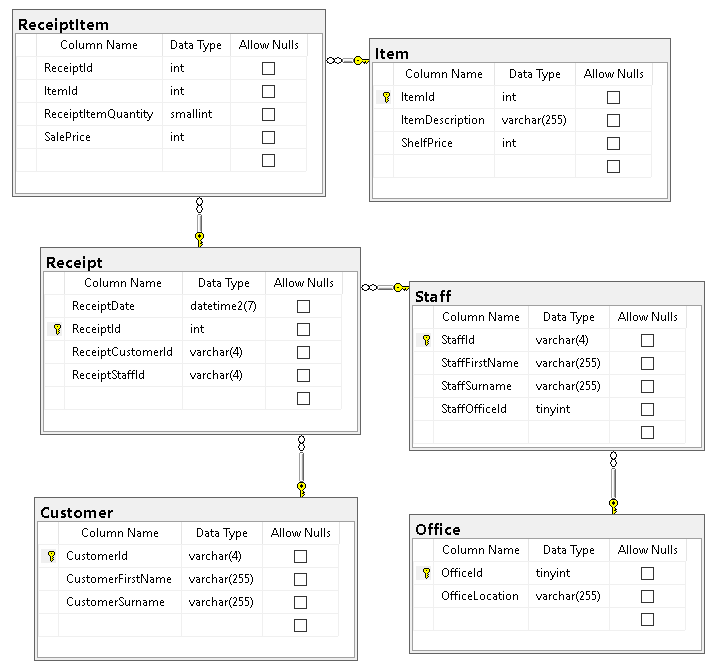
\includegraphics[width=\textwidth,keepaspectratio]{Images/schema.PNG}
                \end{center}
            It must be noted that the structure of this data model is 
            less than efficient, and it would be expected in a datamart
            situation that only at lower levels of data would this schema
            remain responsive in the manner it is now, as the outline
            suggests the datamart is not necessarily the most suitable
            design for future use, however suits very well currently.
            \par
            It would be expected that only at extremely large data sets
            would this model prove a bad design. In such cases a model 
            more representative of the snowflake or star schema would be
            heavily advised.

%%%%%%%%%%%%%%%%%
\newpage
%%%%%%%%%%%%%%%%%

        \subsection{EER Diagram}
            An EER diagram of the suggested data model is provided below. 

            \bigskip

            \begin{center}
                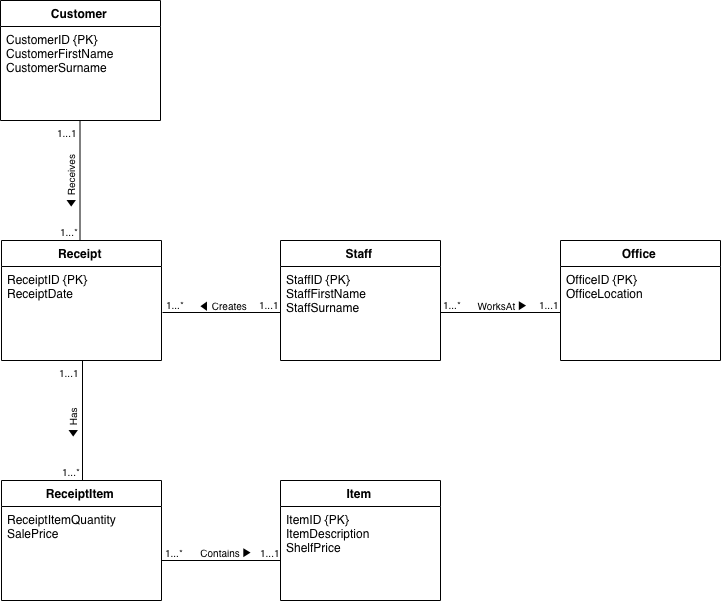
\includegraphics[width=\textwidth-40pt,keepaspectratio]{Images/A2-EERModel.png}
            \end{center}

% ------------------------------------------------------------------------------------------------ %
% DATA LOAD PROCESS
% ------------------------------------------------------------------------------------------------ %

%%%%%%%%%%%%%%%%%
\newpage
%%%%%%%%%%%%%%%%%

    \section{Data Load Process (ETL/ELT)}
    \label{sec:ETL}
        Initial import of the data supplied in the xlsx file generated a very basic table
        that allowed us to analyze the data for potential outliers, confirm the business
        requirements of the data and then create tables from which the data model was derived.
        \\
        The Imported table structure was as follows:
        \begin{center}
            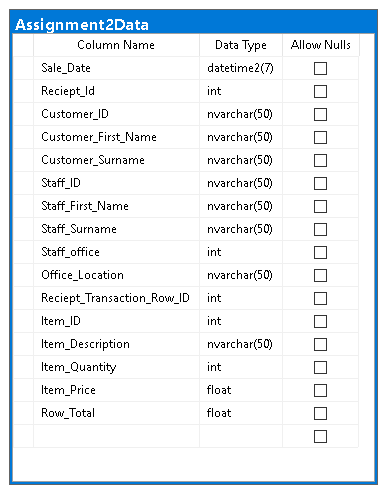
\includegraphics{Images/Initial_Import.PNG}
        \end{center}

        \noindent
        A decision to leave this initial import table as default
        was made to allow easy reference to the initially supplied
        excel data file.

%%%%%%%%%%%%%%%%%
\newpage
%%%%%%%%%%%%%%%%%
        
% ------------------------------------------------------------------------------------------------ %
% QA PROCESS
% ------------------------------------------------------------------------------------------------ %

        \subsection{Quality Assurance Processes}
        \label{sec:QAP}
        After performing a basic query to determine if, like our previous project, multiple 
        items of the same ID on a single receipt existed it was 
        apparent that the same issue existed in this data set as did in the previous.
        \\
        To mitigate this, the team developed a simple update to the 
        ReceiptItem was performed, to ensure that a dicount would not be applied to a receipt with 
        less than five items, when potentially the receipt did not 
        actually have more than four distinct items.
        The following query was used to determine this information:
        \begin{lstlisting}
        -- Verify that no receipt has duplicate ItemIds and all are unique per order
        SELECT *
        FROM
        (
            SELECT [ReceiptItem].[ReceiptId], 
            COUNT([ReceiptItem].[ReceiptId]) AS 'ItemCount',
            COUNT(DISTINCT [ReceiptItem].[ItemId]) AS 'ItemIdCount'
            FROM [ReceiptItem]
            GROUP BY [ReceiptItem].[ReceiptId]) AS SubQuery 
        WHERE [SubQuery].[ItemIdCount] != [SubQuery].[ItemCount]
        \end{lstlisting}

        Returning no entries once the data was cleaned with a 
        \hyperref[sec:sharpccleaning]{\color{blue}C\# Script} internally developed.
        This took into account not only checking for data integrity
        but generated new sql to facilitate \hyperref[sec:sharpcsqlgeneration]{\color{blue}item consolidation}.
        These scripts have been listed in the appendices of this report.

%%%%%%%%%%%%%%%%%
\newpage
%%%%%%%%%%%%%%%%%

% ------------------------------------------------------------------------------------------------ %
% ASSUMPTIONS/REASONING
% ------------------------------------------------------------------------------------------------ %

        \subsection{Assumptions and Reasoning}
        \label{sec:AR}
		The following section outlines our assumptions and the reasoning behind certain decisions
		made by the team at any stage of the project. The team will always try to apply business
		rules supplied by the firm to any of the decisions made however this is not always possible.
		In this case, the reasoning has been listed in the section that follows.        
        
            \subsubsection{Item}
                There were no major assumptions made for the items.
                We followed the feedback received from the previous project 
                and used the associative entity of ReceiptItem
                to satisfy requirements of sale price and quantity.

            \subsubsection{ReceiptItem}
                As suggested above, the ReceiptItem table was created
                to satisfy feedback received on our previous project
                , allows for quantity and price association.

            \subsubsection{Receipt}
                The receipt had no changes in comparison to the previous
                analysis, the changes occured in related entities 
                and did not affect the receipt table.

            \subsubsection{Staff}
                Staff were left untouched, the relation to location 
                however did play a large role in this analysis, and 
                a major assumption of a staff member only being at one 
                location at a time or being directly related only to
                the one location was made.
                \\
                This assumption normally would not be made, but 
                assurances of data cleanliness were made, and the C\#
                script did not find any discrepencies between our assumption and the supplied information.

            \subsubsection{Customer}
            \sout{We made assumptions that customers are likely to shop at only the one store. Given the geographic distances
                between stores generally being larger than we deemed 
                most people would be likely to travel.}
                This assumption was quickly invalidated as most customers 
                seem to have shopped at most if not all stores.

            \subsubsection{Office}
                Our analysis assumed future office potential growth to be 
                related to the locality of the store. Such an assumption
                may suggest that we weighed in favour of stores in 
                high population areas if the analysis was borderline
                for example: Newcastle and Broken Hill; Newcastle
                would be favoured as the growth potential was assumed to 
                be greater and more predictable into the future.

%%%%%%%%%%%%%%%%%
\newpage
%%%%%%%%%%%%%%%%%

% ------------------------------------------------------------------------------------------------ %
% BASE ANALYSIS
% ------------------------------------------------------------------------------------------------ %
    \section{Base Analysis}
    \label{sec:BA}

        \subsection{Notes on Analysis}
            Analysis was performed using Microsoft SQL Management Studio,
            with a flat file of the original data being imported into 
            the table as defined \hyperref[sec:ETL]{\color{blue}here},
            as with the previous assignment utilisation of decimal(18.7) was our choice over using the money type, again citing
            the imprecision of money in MSSQL/TSQL\cite{MoneyIssues}

            Source files to immitate the analysis below is either included inline or in sources files in the final submission.

            \subsection{Raw Results}

            \subsubsection{Total Revenue Per Store}
            The total revenue per store after discounts were applied was determined by the following 
            query:
            \begin{lstlisting}
            -- Item Count, total revenue, sold By Office Location with discount
            SELECT (CAST(
                    CASE
                    WHEN COUNT(ri.[ReceiptItemQuantity]) >= 5
                        THEN SUM(ri.[SalePrice] * ri.[ReceiptItemQuantity]) * 0.95
                    ELSE SUM(ri.[SalePrice] * ri.[ReceiptItemQuantity])
                    END AS decimal(19,5))) AS 'Revenue',
            o.OfficeId, o.OfficeLocation
            FROM Receipt r
                INNER JOIN ReceiptItem ri
                            ON r.ReceiptId = ri.ReceiptId
                INNER JOIN Staff s
                            ON s.StaffId = r.ReceiptStaffId
                INNER JOIN Office o
                            ON s.StaffOfficeId = o.OfficeId
            GROUP BY o.OfficeId
                    , o.OfficeLocation
            ORDER BY Revenue DESC;
            \end{lstlisting}
            With results:
            \begin{table}[H]
                \centering
                \begin{tabular}{|l|l|l|}
                \hline
                Revenue       & OfficeId & OfficeLocation \\ \hline
                \$1807157.30 & 9        & Wagga Wagga    \\ \hline
                \$1243761.42 & 2        & Maitland       \\ \hline
                \$1206763.76 & 10       & Broken Hill    \\ \hline
                \$1113333.40 & 4        & Sydney         \\ \hline
                \$1109330.77 & 1        & Newcastle      \\ \hline
                \$1092924.88 & 5        & Port Macquarie \\ \hline
                \$1006184.56 & 3        & Cessnock       \\ \hline
                \$1001501.30 & 6        & Grafton        \\ \hline
                \$934267.47  & 7        & Dubbo          \\ \hline
                \$891871.68  & 8        & Wollongong     \\ \hline
                \end{tabular}
            \end{table}

%%%%%%%%%%%%%%%%%
\newpage
%%%%%%%%%%%%%%%%%

            \subsubsection{Total Number of Sales}
                The total number of sales per staff member were considered with the following 
                sql query:
                \begin{lstlisting}
				SELECT COUNT(*) AS 'Sales Count'
						, s.StaffId
						, s.StaffFirstName
						, s.StaffSurname
						, o.OfficeId
						, o.OfficeLocation
				FROM Receipt r
					INNER JOIN ReceiptItem ri
								 ON r.ReceiptId = ri.ReceiptId
					INNER JOIN Item i
								 ON i.ItemId = ri.ItemId
					INNER JOIN Staff s
								 ON s.StaffId = r.ReceiptStaffId
					INNER JOIN Office o
								 ON o.OfficeId = s.StaffOfficeId
				GROUP BY s.StaffId
						, s.StaffFirstName
						, s.StaffSurname
						, o.OfficeId
						, o.OfficeLocation
				ORDER BY 'Sales Count' DESC;
                \end{lstlisting}

                \begin{table}[H]
                    \centering
                    \begin{tabular}{|l|l|l|l|l|l|}
                    \hline
                    Sales Count & StaffId & StaffFirstName & StaffSurname & OfficeId & OfficeLocation \\ \hline
                    645         & S190    & Samuel         & Anderson     & 4        & Sydney         \\ \hline
                    628         & S196    & Devin          & Brown        & 6        & Grafton        \\ \hline
                    628         & S122    & Austin         & Morris       & 6        & Grafton        \\ \hline
                    608         & S101    & Jenna          & Cox          & 5        & Port Macquarie \\ \hline
                    607         & S45     & Emma           & Gutierrez    & 3        & Cessnock       \\ \hline
                  \end{tabular}
                \end{table}
                
                \noindent
                This suggests to us that select stores had more either more sales or 
                higher performing employees, which we wanted to confirm in analysis later, of which can be found here.

%%%%%%%%%%%%%%%%%
\newpage
%%%%%%%%%%%%%%%%%

            \subsubsection{Total Items Sold}
                The total items attributed to each staff member were considered also,
                determined by the query:
                
                \begin{lstlisting}
				SELECT SUM(ri.ReceiptItemQuantity) AS 'Item Count'
						, s.StaffId
						, s.StaffFirstName
						, s.StaffSurname
						, o.OfficeId
						, o.OfficeLocation
				FROM Receipt r
					INNER JOIN ReceiptItem ri
									 ON r.ReceiptId = ri.ReceiptId
					INNER JOIN Staff s
									 ON s.StaffId = r.ReceiptStaffId
					INNER JOIN Office o
									 ON o.OfficeId = s.StaffOfficeId
				GROUP BY s.StaffId
						, s.StaffFirstName
						, s.StaffSurname
						, o.OfficeId
						, o.OfficeLocation
				ORDER BY 'Item Count' DESC;
                \end{lstlisting}

                % Yielding a range of 4217 to 2813, with the top five staff members in this
                % analysis:

                \begin{table}[H]
                    \centering
                    \begin{tabular}{|l|l|l|l|l|l|}
                    \hline
                    Item Count & StaffId & StaffFirstName & StaffSurname & OfficeId & OfficeLocation \\ \hline
                    4005       & S190    & Samuel         & Anderson     & 4        & Sydney         \\ \hline
                    3796       & S122    & Austin         & Morris       & 6        & Grafton        \\ \hline
                    3730       & S101    & Jenna          & Cox          & 5        & Port Macquarie \\ \hline
                    3716       & S45     & Emma           & Gutierrez    & 3        & Cessnock       \\ \hline
                    3684       & S108    & Isaiah         & Powell       & 9        & Wagga Wagga    \\ \hline
                    \end{tabular}
                    \end{table}

%%%%%%%%%%%%%%%%%
\newpage
%%%%%%%%%%%%%%%%%
                    
            \subsubsection{Discounted Sales Ratio}
                Consideration of the number of sales made by each staff member was also made,
                the following query yielding the results we required:

            \begin{lstlisting}
				SELECT s.StaffId
						, s.StaffFirstName
						, s.StaffSurname
						, o.OfficeId
						, o.OfficeLocation
						, SUM(SubQuery.[Discounted Sales]) AS 'Discounted Sales'
						, SUM(SubQuery.[Standard Sales]) AS 'Standard Sales'
				FROM (
					SELECT CAST(
						CASE
						WHEN COUNT(ri.[ReceiptItemQuantity]) >= 5
							THEN 1
						ELSE 0
						END AS INT) AS 'Discounted Sales',
					CAST(
						CASE
						WHEN COUNT(ri.[ReceiptItemQuantity]) >= 5
							THEN 0
						ELSE 1
					END AS INT) AS 'Standard Sales',
					r.ReceiptId
					FROM Receipt r
						INNER JOIN ReceiptItem ri
									 ON r.ReceiptId = ri.ReceiptId
						INNER JOIN Item i
									 ON i.ItemId = ri.ItemId
					GROUP BY r.ReceiptId
				) AS SubQuery
					INNER JOIN Receipt r
								 ON SubQuery.ReceiptId = r.ReceiptId
					INNER JOIN ReceiptItem ri
								 ON r.ReceiptId = ri.ReceiptId
					INNER JOIN Staff s
								 ON s.StaffId = r.ReceiptStaffId
					INNER JOIN Office o
								 ON o.OfficeId = s.StaffOfficeId
				GROUP BY s.StaffId
						, s.StaffFirstName
						, s.StaffSurname
						, o.OfficeId
						, o.OfficeLocation
				ORDER BY [Discounted Sales];
            \end{lstlisting}

            \begin{table}[H]
                \centering
                \begin{tabular}{|l|l|l|l|l|l|l|}
                \hline
                StaffId & StaffFirstName & StaffSurname & OfficeId & OfficeLocation & Discounted Sales & Standard Sales \\ \hline
                S51     & Haley          & Taylor       & 7        & Dubbo          & 263              & 91             \\ \hline
                S161    & Jason          & Wood         & 7        & Dubbo          & 273              & 117            \\ \hline
                S17     & Daniel         & Baker        & 1        & Newcastle      & 278              & 112            \\ \hline
                S135    & Lexi           & James        & 4        & Sydney         & 280              & 100            \\ \hline
                S73     & John           & White        & 2        & Maitland       & 286              & 121            \\ \hline
                \end{tabular}
                \end{table}


%%%%%%%%%%%%%%%%%
\newpage
%%%%%%%%%%%%%%%%%

            \subsubsection{Total Sales Value per Staff Member}

            % Consideration of the total sales per staff member was considered a highly important 
            % metric to consider also, we did consider comparing the results of this to the 
            % results of a query that did not include discount to see whom would be considered
            % the best performer if discounts were not relevant, however we also recognise this to be too
            % speclutive in nature. The required query was as follows:

            \begin{lstlisting}
				SELECT CAST(
						CASE
						WHEN COUNT(ri.[ReceiptItemQuantity]) >= 5
							THEN SUM(ri.[SalePrice] * ri.[ReceiptItemQuantity]) * 0.95
						ELSE SUM(ri.[SalePrice] * ri.[ReceiptItemQuantity])
						END AS decimal(19,5)) AS 'Sales Totals'
						, s.StaffId
						, s.StaffFirstName
						, s.StaffSurname
						, o.OfficeId
						, o.OfficeLocation
				FROM Receipt r
					INNER JOIN ReceiptItem ri
								ON r.ReceiptId = ri.ReceiptId
					INNER JOIN Item i
								ON i.ItemId = ri.ItemId
					INNER JOIN Staff s
								ON s.StaffId = r.ReceiptStaffId
					INNER JOIN Customer c
								ON c.CustomerId = r.ReceiptCustomerId
					INNER JOIN Office o
								ON o.OfficeId = s.StaffOfficeId
				GROUP BY s.StaffId
						, s.StaffFirstName
						, s.StaffSurname
						, o.OfficeId
						, o.OfficeLocation
				ORDER BY 'Sales Totals' DESC;
            \end{lstlisting}

            \begin{table}[H]
                \centering
                \begin{tabular}{|l|l|l|l|l|l|}
                \hline
                Sales Totals & StaffId & StaffFirstName & StaffSurname & OfficeId & OfficeLocation \\ \hline
                \$77152.49  & S187    & Savannah       & Jones        & 8        & Wollongong     \\ \hline
                \$75113.60  & S45     & Emma           & Gutierrez    & 3        & Cessnock       \\ \hline
                \$72475.45  & S178    & Kaitlyn        & Nguyen       & 2        & Maitland       \\ \hline
                \$71814.20  & S122    & Austin         & Morris       & 6        & Grafton        \\ \hline
                \$71497.09  & S71     & Danielle       & Myers        & 6        & Grafton        \\ \hline
                \end{tabular}
                \end{table}

%%%%%%%%%%%%%%%%%
\newpage
%%%%%%%%%%%%%%%%%

            \subsubsection{Average Value Per Sale}

            % The average receipt value per staff member was another metric we considered would add
            % value to the descision to be suggested in the 
            % \hyperref[sec:Executive Summary]{\color{blue}executive summary}.
            % The required query to determine this metric was as follows:

            \begin{lstlisting}
				SELECT (CAST(
						CASE
						WHEN COUNT(ri.[ReceiptItemQuantity]) >= 5
							THEN SUM(ri.[SalePrice] * ri.[ReceiptItemQuantity]) * 0.95
						ELSE SUM(ri.[SalePrice] * ri.[ReceiptItemQuantity])
						END AS decimal(19,5)) / COUNT(r.ReceiptId)) AS 'Sales Average'
						, s.StaffId
						, s.StaffFirstName
						, s.StaffSurname
						, o.OfficeId
						, o.OfficeLocation
					FROM Receipt r
					INNER JOIN ReceiptItem ri
									 ON r.ReceiptId = ri.ReceiptId
					INNER JOIN Item i
									 ON i.ItemId = ri.ItemId
					INNER JOIN Staff s
									 ON s.StaffId = r.ReceiptStaffId
					INNER JOIN Office o
									 ON o.OfficeId = s.StaffOfficeId
				GROUP BY s.StaffId
						, s.StaffFirstName
						, s.StaffSurname
						, o.OfficeId
						, o.OfficeLocation
				ORDER BY 'Sales Average' DESC;
            \end{lstlisting}

            \begin{table}[H]
                \centering
                \begin{tabular}{|l|l|l|l|l|l|}
                \hline
                Sales Average        & StaffId & StaffFirstName & StaffSurname & OfficeId & OfficeLocation \\ \hline
                \$138.40 & S109    & Nicole         & Hernandez    & 10       & Broken Hill    \\ \hline
                \$134.88 & S187    & Savannah       & Jones        & 8        & Wollongong     \\ \hline
                \$134.71 & S52     & Isabella       & Rivera       & 5        & Port Macquarie \\ \hline
                \$134.53 & S165    & Marcus         & Ross         & 2        & Maitland       \\ \hline
                \$134.12 & S199    & Maria          & Smith        & 5        & Port Macquarie \\ \hline
                \end{tabular}
            \end{table}

            % \par\noindent
             
            % With results as follows:
            % We consider this to be a metric which weighs heavily in our analysis,
            % as multiple factors would impact this result, the number of items on the sale
            % (resulting in a lower total if discount was applied). Another consideration 
            % for this metric would be that it leans towards anyone who could
            % sell a larger quantity of the same item, as this lends itself towards a higher
            % receipt total. 
            
%%%%%%%%%%%%%%%%%
\newpage
%%%%%%%%%%%%%%%%%

            \subsection{Total Items and Revenue per Store}
               
                \begin{lstlisting}
                -- Item Count, total revenue, sold By Office Location with discount
                SELECT (CAST(
                        CASE
                        WHEN COUNT(ri.[ReceiptItemQuantity]) >= 5
                            THEN SUM(ri.[SalePrice] * ri.[ReceiptItemQuantity]) * 0.95
                        ELSE SUM(ri.[SalePrice] * ri.[ReceiptItemQuantity])
                        END AS decimal(19,5))) AS 'Revenue',
                SUM(ri.ReceiptItemQuantity) AS ItemCount,
                o.OfficeId, o.OfficeLocation
                FROM Receipt r
                    INNER JOIN ReceiptItem ri
                                ON r.ReceiptId = ri.ReceiptId
                    INNER JOIN Staff s
                                ON s.StaffId = r.ReceiptStaffId
                    INNER JOIN Office o
                                ON s.StaffOfficeId = o.OfficeId
                GROUP BY o.OfficeId
                        , o.OfficeLocation
                ORDER BY ItemCount DESC;
                \end{lstlisting}

                \begin{table}[H]
                    \centering
                    \begin{tabular}{|l|l|l|l|}
                    \hline
                    Revenue       & ItemCount & OfficeId & OfficeLocation \\ \hline
                    \$1807157.30 & 97020     & 9        & Wagga Wagga    \\ \hline
                    \$1243761.42 & 65637     & 2        & Maitland       \\ \hline
                    \$1206763.76 & 65568     & 10       & Broken Hill    \\ \hline
                    \$1109330.77 & 59946     & 1        & Newcastle      \\ \hline
                    \$1113333.40 & 59229     & 4        & Sydney         \\ \hline
                    \$1092924.88 & 56429     & 5        & Port Macquarie \\ \hline
                    \$1006184.56 & 52315     & 3        & Cessnock       \\ \hline
                    \$1001501.30 & 51533     & 6        & Grafton        \\ \hline
                    \$934267.47  & 49456     & 7        & Dubbo          \\ \hline
                    \$891871.68  & 46433     & 8        & Wollongong     \\ \hline
                    \end{tabular}
                \end{table}

%%%%%%%%%%%%%%%%%
\newpage
%%%%%%%%%%%%%%%%%

            \subsection{Unique Customers Per Store}
                
            Total number of customers per store were determine via the below query:

            \begin{lstlisting}
                -- Unique Customer Count Per Store
                SELECT COUNT(*) AS 'Customer Count', o.[OfficeLocation]
                FROM Customer c
                INNER JOIN Receipt r ON r.ReceiptCustomerId = c.CustomerId
                INNER JOIN Staff s ON s.StaffId = r.ReceiptStaffId
                INNER JOIN Office o ON o.OfficeId = s.StaffOfficeId
                GROUP BY o.[OfficeLocation]
                ORDER BY 'Customer Count' DESC;
            \end{lstlisting}

            \begin{table}[H]
                \centering
                \begin{tabular}{|l|l|}
                \hline
                Customer Count & OfficeLocation \\ \hline
                600            & Wagga Wagga    \\ \hline
                584            & Maitland       \\ \hline
                581            & Port Macquarie \\ \hline
                581            & Broken Hill    \\ \hline
                577            & Sydney         \\ \hline
                574            & Newcastle      \\ \hline
                571            & Cessnock       \\ \hline
                564            & Dubbo          \\ \hline
                559            & Grafton        \\ \hline
                556            & Wollongong     \\ \hline
                \end{tabular}
            \end{table}

            \noindent
            This suggests that customers generally will shop at a number of stores, not just the single store in their locality, however being an online business 
            and knowing that the unique pool of customers in this dataset was 600 
            also suggests that a customer can order from anywhere and have the item
            delivered or transfered to a local store potentially.
            \\
            Given this, we assume that closing a store will not greatly impact 
            customer retention if an online outlet can be reached.

%%%%%%%%%%%%%%%%%
\newpage
%%%%%%%%%%%%%%%%%

            \subsection{Item Popularity}
            Top 3 best and worst items overall, correlation to any stores?

            \begin{lstlisting}
                SELECT SUM(ri.ReceiptItemQuantity) AS ItemCount
                , i.ItemId
                , i.ItemDescription
                , o.OfficeId
                , o.OfficeLocation
                    FROM Receipt r
                        INNER JOIN ReceiptItem ri
                                    ON ri.ReceiptId = r.ReceiptId
                        INNER JOIN Item i
                                    on i.ItemId = ri.ItemId
                        INNER JOIN Staff s
                                    on s.StaffId = r.ReceiptStaffId
                        INNER JOIN Office o
                                    on o.OfficeId = s.StaffOfficeId
                    WHERE o.OfficeId = 1
                    GROUP BY i.ItemId
                            , i.ItemDescription
                            , o.OfficeId
                            , o.OfficeLocation
                    ORDER BY ItemCount ASC;
            \end{lstlisting}

            \begin{table}[H]
                \centering
                \begin{tabular}{|l|l|l|l|l|l|l|}
                \hline
                Office ID & Item ID & Highest Quality 1 & Item ID & Highest Quality 2 & Item ID & Highest Quality 3  \\ \hline
                1         & 24      & 2144              & 13      & 2153              & 26      & 2176               \\ \hline
                2         & 7       & 2328              & 28      & 2371              & 5       & 2374               \\ \hline
                3         & 10      & 1885              & 18      & 1900              & 22      & 2144               \\ \hline
                4         & 16      & 2151              & 20      & 2157              & 4       & 2185               \\ \hline
                5         & 20      & 2038              & 27      & 2042              & 10      & 2051               \\ \hline
                6         & 25      & 1846              & 16      & 1856              & 2       & 1881               \\ \hline
                7         & 20      & 1807              & 30      & 1808              & 24      & 1864               \\ \hline
                8         & 5       & 1674              & 8       & 1696              & 16      & 1765               \\ \hline
                9         & 25      & 3405              & 21      & 3478              & 14      & 3566               \\ \hline
                10        & 14      & 2376              & 22      & 2384              & 8       & 2436               \\ \hline
                \end{tabular}
                \end{table}


            \begin{table}[H]
                \centering
                \begin{tabular}{|l|l|l|l|l|l|l|}
                \hline
                Office ID & Item ID & Lowest Quality 1 & Item ID & Lowest Quality 2 & Item ID & Lowest Quality 3  \\ \hline
                1         & 11      & 1756             & 2       & 1765             & 17      & 1866              \\ \hline
                2         & 27      & 1947             & 9       & 1966             & 2       & 2027              \\ \hline
                3         & 5       & 1465             & 8       & 1500             & 27      & 1561              \\ \hline
                4         & 23      & 1767             & 13      & 1810             & 14      & 1829              \\ \hline
                5         & 1       & 1563             & 8       & 1663             & 6       & 1680              \\ \hline
                6         & 29      & 1537             & 20      & 1562             & 17      & 1573              \\ \hline
                7         & 25      & 1397             & 4       & 1471             & 2       & 1494              \\ \hline
                8         & 14      & 1383             & 17      & 1422             & 24      & 1424              \\ \hline
                9         & 16      & 2945             & 23      & 3001             & 28      & 3010              \\ \hline
                10        & 5       & 1939             & 11      & 1962             & 13      & 1980              \\ \hline
                \end{tabular}
                \end{table}

%%%%%%%%%%%%%%%%%
\newpage
%%%%%%%%%%%%%%%%%

            \subsection{Worst Performing Item}
                Correlation to store?

                \begin{lstlisting}
                    --worst perfroming items for the company as whole
                    SELECT SUM(ri.ReceiptItemQuantity) AS ItemCount
                            , i.ItemId
                            , i.ItemDescription
                    FROM Receipt r
                        INNER JOIN ReceiptItem ri
                                    ON ri.ReceiptId = r.ReceiptId
                        INNER JOIN Item i
                                    ON i.ItemId = ri.ItemId
                    GROUP BY i.ItemId, i.ItemDescription
                    ORDER BY ItemCount ASC;
                \end{lstlisting}

                \begin{table}[H]
                    \centering
                    \begin{tabular}{|l|l|l|l|}
                    \hline
                    ItemCount & ItemId & ItemDescription \\ \hline
                    19481     & 23     & Drill Bit 6mm   \\ \hline
                    19613     & 13     & Ruler           \\ \hline
                    19741     & 2      & Screwdriver Set \\ \hline
                    19744     & 9      & Box of Screws   \\ \hline
                    19746     & 17     & Punch           \\ \hline
                    \end{tabular}
                    \end{table}

% ------------------------------------------------------------------------------------------------ %
% CONCLUSION & RECOMMENDATIONS
% ------------------------------------------------------------------------------------------------ %
%%%%%%%%%%%%%%%%%
\newpage
%%%%%%%%%%%%%%%%%

    \section{Conclusion and Recommendations}
            % This report is designed to identify the best performing Sales Officer at BIA Inc by 
            % directive of the Head Sales Executive of BIA Inc.
            % After considering multiple data points from the newly created Sales Database, 
            % using sales data from 2017 supplied to us by the Head Sales Executive of BIA Inc.
            % We conclude that the Best Sales Officer is Mrs Michelle Miller (S8) becasue she 
            % has a sales total of \$78,572.22 more than \$4k more than the second highest 
            % revenue maker Mrs Kaitlyn Ortiz (S19).
            % She does not have the Highest transaction count however because she has sold 
            % more higher value items this makes up for it. She has sold 4144 compared to 
            % the highest count of 4217. It works out to be a 73 item difference.
            % We beleive that the in excess of \$4k extra that Mrs Michelle Miller brings 
            % to the company out weighs the value of selling 73 extra items. 
            % There for we recommend Mrs Michelle Miller for the reward as the best Sales 
            % Officer at BIA Inc. In the event that  Mrs Michelle Miller is not applicable
            % we would reccomend Mrs Kaitlyn Ortiz whom has 
			% achieved a high evaluation from all the data points that we analyzed.

% ------------------------------------------------------------------------------------------------ %
% REFERENCES
% ------------------------------------------------------------------------------------------------ %
    
%%%%%%%%%%%%%%%%%
\newpage
%%%%%%%%%%%%%%%%%

    \begin{thebibliography}{9}
        \raggedright
        \bibitem{MoneyIssues}
            Reasons against TSQL Money type: Stackoverflow User; \textit{SQLMenace}
            \url{https://stackoverflow.com/questions/582797/should-you-choose-the-money-or-decimalx-y-datatypes-in-sql-server}
        \bibitem{Numeric}
            Microsoft TSQL documentation of Decimal/Numeric types
            \url{https://docs.microsoft.com/en-us/sql/t-sql/data-types/decimal-and-numeric-transact-sql?view=sql-server-2017}
        \bibitem{CTE}
        Microsoft documentation: WITH common\_table\_expression (Transact-SQL)
            \url{https://docs.microsoft.com/en-us/sql/t-sql/queries/with-common-table-expression-transact-sql?view=sql-server-2017}
        \bibitem{BusDictionairyUpselling}
        		Upselling - Business Dictionary
        		\url{http://www.businessdictionary.com/definition/upselling.html}
    \end{thebibliography}

% ------------------------------------------------------------------------------------------------ %
% APPENDIX
% ------------------------------------------------------------------------------------------------ %

%%%%%%%%%%%%%%%%%
\newpage
%%%%%%%%%%%%%%%%%

    \section{Appendix}
    \label{sec:Appendix}

    \subsection{C\# Code Excerpt: Cleaning}
    \label{sec:sharpccleaning}
    \lstset{style=sharpc}
    \begin{lstlisting}
        public Tuple<Dictionary<int, Receipt>, Dictionary<int, Receipt>, int> GenerateReceipts(DataSet dataSet)
        {
            var receipts = new Dictionary<int, Receipt>();
            var invalidReceipts = new Dictionary<int, Receipt>();
            var counter = 0;

            // Iterate over each sheet in the dataset, in our case it's only one anyway.
            foreach (DataTable table in dataSet.Tables)
                // Iterate over each row in the dataset, it seems this iterates until it finds row with no values in any column.
                foreach (DataRow row in table.Rows)
                {
                    // Ignore the header of the table
                    if (counter > 0)
                    {
                        // Generation of receipt from dataset, ignoring transaction row id as it is not 
                        // relevant and we are consolidating the duplicate items into total quantities anyway. 
                        var receipt = new Receipt
                        {
                            Id = Convert.ToInt32(row[1]),
                            Customer = new Customer
                            {
                                FirstName = row[3].ToString(),
                                Id = row[2].ToString(),
                                Surname = row[4].ToString()
                            },
                            Staff = new Staff
                            {
                                OfficeId = Convert.ToInt32(row[8]),
                                Id = row[5].ToString(),
                                FirstName = row[6].ToString(),
                                Surname = row[7].ToString()
                            },
                            SaleDate = (DateTime)row[0],
                            Items = new Dictionary<int, Item>
                        {
                            {
                                Convert.ToInt32(row[11]), new Item
                                {
                                    Id = Convert.ToInt32(row[11]),
                                    Description = row[12].ToString(),
                                    Price = (double) row[14],
                                    Quantity = Convert.ToInt32(row[13])
                                }
                            }
                        },
                            Office = new Office
                            {
                                Id = Convert.ToInt32(row[8]),
                                OfficeLocation = ParseEnum<Location>(row[9].ToString())
                            }
                        };





                        // Check if receipts either is empty or doesn't have a receipt 
                        // with the same receipt id already, if so add the receipt to 
                        // receipts.
                        if (receipts.Count == 0 || !receipts.ContainsKey(receipt.Id))
                        {
                            AddToReceipts(receipts, receipt);
                            Console.WriteLine($@"Added new receipt: {receipt.Id}");
                        }
                        // 
                        else if (receipts.ContainsKey(receipt.Id))
                        {
                            var existingReceipt = receipts[receipt.Id];

                            // Be warned; below is a fucking mess.

                            // Check all staff properties match the existing receipt properties.
                            if (existingReceipt.Staff.Id != receipt.Staff.Id
                                || existingReceipt.Staff.FirstName != receipt.Staff.FirstName
                                || existingReceipt.Staff.Surname != receipt.Staff.Surname)
                            {
                                AddToReceipts(invalidReceipts, receipt);
                                Console.WriteLine($"Staff Id mismatch on receipt: {existingReceipt.Id}, " +
                                                  $"Staff Ids: {existingReceipt.Staff.Id} and {receipt.Staff.Id}, " +
                                                  $"Staff Names: {existingReceipt.Staff.FirstName} and {receipt.Staff.FirstName}, " +
                                                  $"Staff Surnames: {existingReceipt.Staff.Surname} and {receipt.Staff.Surname}, ");
                                continue;
                            }

                            // Check all office properties match the existing receipt properties.
                            if (existingReceipt.Office.Id != receipt.Office.Id
                                || existingReceipt.Office.OfficeLocation != receipt.Office.OfficeLocation)
                            {
                                AddToReceipts(invalidReceipts, receipt);
                                Console.WriteLine($"Office Id mismatch on receipt: {existingReceipt.Id}, " +
                                              $"Office Ids: {existingReceipt.Office.Id} and {receipt.Office.Id}, " +
                                              $"Office Locations: {existingReceipt.Office.OfficeLocation} and {receipt.Office.OfficeLocation}");
                                continue;
                            }

                            // Check all date properties match the existing receipt properties.
                            if (existingReceipt.SaleDate != receipt.SaleDate)
                            {
                                AddToReceipts(invalidReceipts, receipt);
                                Console.WriteLine($"Sale date mismatch on receipt: {existingReceipt.Id}, " +
                                                  $"Dates: {existingReceipt.SaleDate} and {receipt.SaleDate}");
                                continue;
                            }











                            // Check all customer properties match the existing receipt properties.
                            if (existingReceipt.Customer.Id != receipt.Customer.Id
                                || existingReceipt.Customer.FirstName != receipt.Customer.FirstName
                                || existingReceipt.Customer.Surname != receipt.Customer.Surname)
                            {
                                AddToReceipts(invalidReceipts, receipt);
                                Console.WriteLine($"Customer mismatch on receipt: {existingReceipt.Id}, " +
                                                  $"Customers Ids: {existingReceipt.Customer.Id} and {receipt.Customer.Id}, " +
                                                  $"Customers Names: {existingReceipt.Customer.FirstName} and {receipt.Customer.FirstName}, " +
                                                  $"Customers Surnames: {existingReceipt.Customer.Surname} and {receipt.Customer.Surname}, ");
                                continue;
                            }

                            // If not item mismatches exist, we need to determine if the item 
                            // exists in both the compared receipts.
                            var key = receipt.Items.First().Key;
                            var value = receipt.Items.First().Value;

                            // Check if the item exists in the existing receipt already.
                            if (existingReceipt.Items.ContainsKey(receipt.Items.First().Key))
                            {
                                var quantity = receipt.Items.First().Value.Quantity;
                                Console.WriteLine($"Item exists in current receipt with Id: {key}, " +
                                                  $"updated item quantity from: {existingReceipt.Items[key].Quantity} " +
                                                  $"to new quantity: {existingReceipt.Items[key].Quantity + quantity}");

                                // Update quantity on item in existing receipt.
                                existingReceipt.Items[key].Quantity += quantity;
                                receipts[existingReceipt.Id] = existingReceipt;
                            }
                            else
                            {
                                // Update the receipt with the new item added.
                                existingReceipt.Items.Add(key, value);
                                Console.WriteLine($@"Added item with Id: {value.Id} to existing receipt: {receipt.Id}");
                            }
                        }
                    }
                    counter++;
                }

            return new Tuple<Dictionary<int, Receipt>, Dictionary<int, Receipt>, int>(receipts, invalidReceipts,
                counter);
        }
    \end{lstlisting}

%%%%%%%%%%%%%%%%%
\newpage
%%%%%%%%%%%%%%%%%

    \subsection{C\# Code Excerpt: SQL Generation}
    \label{sec:sharpcsqlgeneration}
    \begin{lstlisting}
    public string GenerateSQL(Dictionary<int, Receipt> receipts)
    {
        var output = new StringBuilder();

        foreach(var receipt in receipts)
        {
            var itemTotalPrices = new Dictionary<int, double>();

            foreach (var item in receipt.Value.Items)
            {
                var totalItemPrice = item.Value.Price * item.Value.Quantity;
                itemTotalPrices.Add(item.Key, totalItemPrice);
            };

            var total = itemTotalPrices.Sum(x => x.Value);
            var discountTotal = (itemTotalPrices.Count >= 5) ? total * 0.95 : 0;

            var sql = new StringBuilder($@"


        INSERT INTO [Receipt] 
        VALUES('{receipt.Value.SaleDate.ToString("G",CultureInfo.CreateSpecificCulture("en-us"))}',
                {receipt.Key},
                '{receipt.Value.Customer.Id}',
                '{receipt.Value.Staff.Id}',
                {total},
                {discountTotal});");

            foreach (var item in itemTotalPrices)
            {
                sql.Append($@"

        INSERT INTO [ReceiptItem]
        VALUES( {receipt.Key},
                {item.Key},
                {receipt.Value.Items.Select(x => x.Value).Where(y => y.Id == item.Key).FirstOrDefault().Quantity},
                {receipt.Value.Items.Select(x => x.Value).Where(y => y.Id == item.Key).FirstOrDefault().Price});");
            }

            output.Append(sql);
        };

        return output.ToString();
    }
    \end{lstlisting}
    
    \end{document}